\documentclass[11pt, a4paper]{article}

\usepackage[utf8]{inputenc}
\usepackage{graphicx}
\graphicspath{ {images/} }
\usepackage{mathtools}
\usepackage{amssymb}
\usepackage{amsmath}
\usepackage[ngerman,english]{babel}
\usepackage{cite}
\usepackage{bibgerm}
\usepackage{fullpage}
\usepackage[top=1.5cm,bottom=1.5cm,left=3.5cm,right=2.5cm,headsep=1.5cm,includeheadfoot]{geometry}
\usepackage{tabularx}
\usepackage{caption}
\usepackage{subcaption}
\usepackage{eurosym}
\usepackage{enumitem}
\usepackage{multicol}
\usepackage{tikz}
\usepackage{tkz-euclide}
\usepackage{pgfplots}
\usepackage{pdflscape}
\usepackage{acronym}
\usepackage{blindtext}
\usepackage{ifthen}
\usepackage{setspace}
\usepackage{cancel}
\usepackage{color}
\usepackage{listings}
\usepackage{comment}
\usepackage{xcolor}
\usepackage{colortbl}
\usepackage[parfill]{parskip}
\usepackage{url}

\usepackage{fancyhdr}
\pagestyle{fancy}

\fancyhf{} % clear all
\fancyhead[L]{\leftmark}
\fancyfoot[C]{-- \thepage{} --}
%\setlength{\headheight}{15pt}
\renewcommand{\headrulewidth}{0.5pt}
\renewcommand{\footrulewidth}{0pt}
\setlength{\skip\footins}{0.7cm}

\usetikzlibrary{graphs}
\usetikzlibrary{positioning}

\onehalfspacing
\setlength\parindent{0pt}

%\everymath{\displaystyle}

\allowdisplaybreaks

\definecolor{AI-BLUE}{rgb}{0,0.57,0.87}

% Eigene Befehle
\newcommand\q[1]{\glqq{}#1\grqq{}}
\renewcommand\equiv{\Leftrightarrow}
\newcommand\vertequal[2]{\underset{\underset{#2}{\parallel}}{#1}}
\newcommand\cif{\text{if }}
\newcommand\abs[1]{\left|#1\right|}
\newcommand\norm[1]{\abs{\abs{#1}}}
\newcommand\diff[1]{\text{ d#1}}
\newcommand\av[1]{\left\langle#1\right\rangle}
\newcommand\ev[1]{\mathbb{E}\left(#1\right)}
\newcommand\br[1]{\left(#1\right)}
\newcommand\ubr[2]{\underbrace{#1}_{#2}}
\newcommand\quer[1]{\overline{#1}}
\newcommand\setequal{\overset{!}{=}}
\newcommand\dint{\displaystyle \int}
\newcommand\dsum{\displaystyle \sum}
\newcommand\dprod{\displaystyle \prod}
\newcommand\closedInt[2]{\left[#1,#2\right]}
\newcommand{\checkbox}{\Large \Square \normalsize \hspace{0.4cm}}

\newcommand\myref[1]{\ref{#1} (S. \pageref{#1})}
\newcommand\myrefcomma[1]{\ref{#1}, S. \pageref{#1}}

\begin{document}

\thispagestyle{empty}

\setlength{\hoffset}{-0.5cm} % center title page

\lstset{
  basicstyle=\small,           % the size of the fonts that are used for the code
  breaklines=true,             % sets automatic line breaking
  captionpos=b,                % sets the caption-position to bottom
  frame=single,                % adds a frame around the code
  keepspaces=true,             % keeps spaces in text, useful for keeping indentation of code (possibly needs columns=flexible)
  numbers=right,               % where to put the line-numbers; possible values are (none, left, right)
  showspaces=false,            % show spaces everywhere adding particular underscores; it overrides 'showstringspaces'
  stepnumber=1,                % the step between two line-numbers. If it's 1, each line will be numbered
  tabsize=4,                   % sets default tabsize to 4 spaces
  xleftmargin=0.14cm		   % sets left margin
}


\begin{titlepage}
    \begin{center}
    \vphantom{0cm}
    \LARGE \textbf{Report}\\
    \vspace{3cm}
    \normalsize
    Study Project Report \\
    in the Master Program of \textcolor{AI-BLUE}{[Applied Computerscience]}\\
    at the Ruhr-University Bochum\\
    in the Winter Term 2015/16\\
    \vspace{4cm}
    \huge \textbf{Convolutional Neural Networks} \\
    \vspace{4cm}
    \normalsize
    \textbf{Project Participants}\\
    B. Sc. Christian Andreas Mielers (108 011 204 956)\\
    B. Sc. Phil Yannick Schrör (108 011 214 024)\\
    \vspace{2cm}
    \textbf{Project Supervisor:}\\
    PD Dr. Rolf P. Würtz
    \end{center}
\end{titlepage}

\newpage
\pagenumbering{arabic}
\setcounter{page}{2}

\tableofcontents

\newpage
\section{Introduction}
Convolutional neural networks (CNNs) are powerful tools in the field of machine learning. Their strength results from the efficient use of free parameters by exploiting the spatial structure of their input. Instead of learning every weight in the INPUT $\times$ OUTPUT matrix of a fully connected layer, a convolutional layer learns the weights in filters of a fixed size. Since the filters are generally tiny compared to a full weight matrix, using many filters and layers becomes feasible. The convolution operation with those filters then produces a layer response that indicates the local features represented by the filters.

To reduce the amount of data passed through the network, pooling layers that combine the values in small regions of the input into a single value can be used. One can then think of the consecutive application of convolutional and pooling layers as mechanisms to iteratively integrate features from ever more remote locations of the image into a compact representation. Fully connected layers can then be used on the representations learned by these layers to perform classification of the input.

Since images typically contain a lot of spatial structure, they are well suited for processing by such a CNN. To study and evaluate the properties of CNNs, we considered a network layout described in \cite{multi-column-neural-network-gtsrb}. Multiple networks which consist of three pairs of convolutional and pooling layers followed up with two fully connected layers were combined into a committee to solve the GTSRB challenge described in \cite{gtsrb}. We used the layout of one such network on the GTSRB dataset and two other datasets and measured the resulting accuracy. The filters on the various convolutional layers were visualized. We also transfered the filters learned on the GTSRB dataset to the other datasets and only trained the fully connected layers to evaluate how well they generalize.

\section{Network details}

\section{Experiments with GTSRB}
The GTSRB dataset described in \cite{gtsrb} is a collection of $39209$ images in a training set and $12630$ images in a test set. In total, there are $43$ classes. The images were taken while driving through German streets and cropped to only contain the traffic sign and some boundary around it. For each physical traffic sign there are many images, that vary in distance, angle and occlusion since they were taken while the car was passing them. For each image, annotations exist, that locate the bounding box of the traffic sign. To generate fixed-size images for our network, we extracted only that part given by the bounding box and rescaled it to $48\times48$ pixels. As an additional preprocessing step, contrast normalization was applied to reduce the considerable illumination differences present in the images.

\subsection{Simple setup}
%TODO fix epoch count
A network was trained on all images of the training set for $10$ epochs. On a TODO CPU with TODO RAM, one epochs takes abount 9 hours. The performance development over the epochs is visualized in figure \ref{fig:gtsrb-results}, and the accuracy is given in a table. After achieving $0.9359$ after the first epoch, it rises monotonically and starts to levels off near $0.9640$ after about 6 epochs.

\begin{figure}[h!]
	\centering
	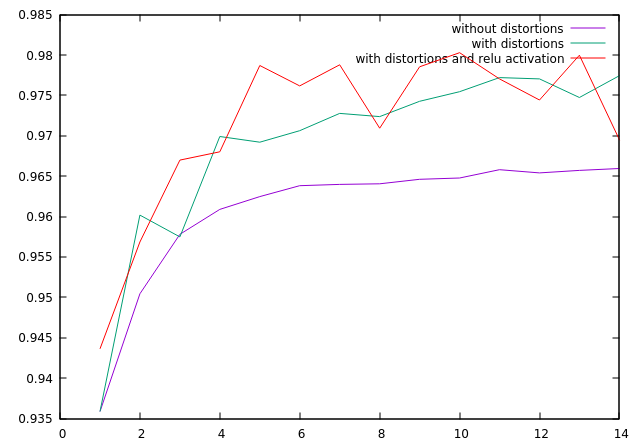
\includegraphics[width=1\textwidth]{gtsrb_results}
	%TODO more epochs in table
	\begin{tabular}{|l|lllllll|}
		\hline
		Epoch & 1 & 2 & 3 & 4 & 5 & 6 & 7\\
		\hline
		without distortions & 0.9359 & 0.9504 & 0.9578 & 0.9609 & 0.9625 & 0.9638 & 0.9640\\
		with distortions & 32 & 33 & 34 & 35 & 36 & 37 & 38\\
		with distortions (relu) & 42 & 43 & 44 & 45 & 46 & 47 & 48\\
		\hline
	\end{tabular}
	\caption{Results of 3 network and training variants on the GTSRB dataset. A network with a $\tanh$ activation function was trained on the data with and without distortions. Additionally, a network with the relu activation function was trained on the continually distorted data.}
	\label{fig:gtsrb-results}
\end{figure}

In the convolutional layers, the network learns filters that are applied to the 3 channels of the color image (in the lowest layer) and to the output of the previous layer (in later cases). Some of these filters are visualized in figure \ref{fig:gtsrb-filters}.

One can observe that the filters on the first layer exhibit a notable spatial structure. In most of them, we see rather broad regions that contain either high or low values. Due to this, one can easily see how they work as feature detectors for the network. They seem to be tuned for edges and corners of various orientations, since this is what the shape of the borders between bright and dark regions mostly suggest. It is also striking that the filters for the 3 channels share a common layout, save for a few details. This indicates that the first layer combines the channels into a unified representation without discriminating between colors. Thus, it seems that the network learns to classify the traffic signs without a lot of dependence on color information. %TODO verify this?

The filters on the higher layers are not so easy to reason about. They have less room to expose structure since they are smaller, but even so there doesn't seem to be a separation between regions of high and low values as strong as on the lowest layer. Since there are a lot of filters for every one of the many input maps to those layers, there is a sizable number of filters involved. This high number of filters might make it useful to increase the specialization of those filters, leading to structures that do not correspond to a visually striking layout. %TODO verify this. Is there more visual structure with fewer filters?

\begin{figure}
	\centering
	\begin{subfigure}{\textwidth}
		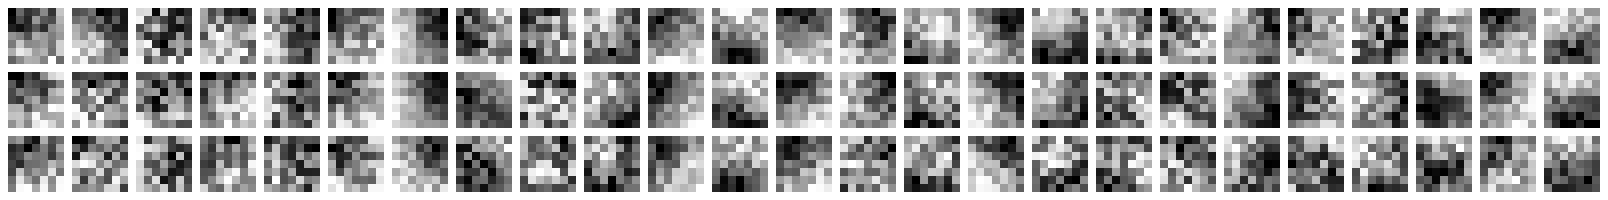
\includegraphics[width=1\textwidth]{filter_visualizations/gtsrb_nomorph_filters_0}
		\caption{Layer 0}
		\label{fig:gtsrb-filters-0}
	\end{subfigure}
	\begin{subfigure}{\textwidth}
		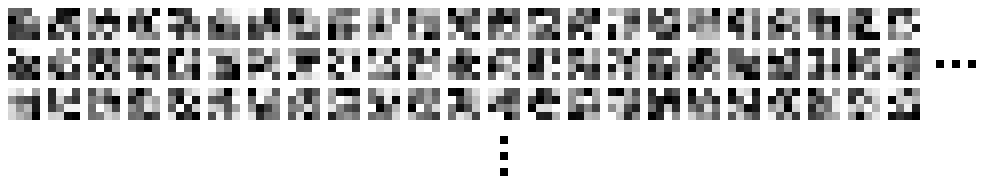
\includegraphics[width=1\textwidth]{filter_visualizations/gtsrb_nomorph_filters_2}
		\caption{Layer 2}
		\label{fig:gtsrb-filters-2}
	\end{subfigure}
	\begin{subfigure}{\textwidth}
		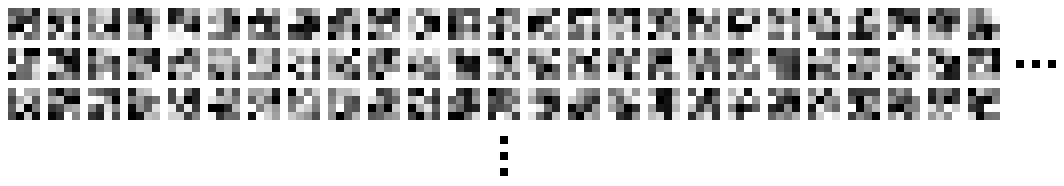
\includegraphics[width=1\textwidth]{filter_visualizations/gtsrb_nomorph_filters_4}
		\caption{Layer 4}
		\label{fig:gtsrb-filters-4}
	\end{subfigure}
	\caption{Filter visualization for the network trained on the original input data after TODO 7 epochs. (\subref{fig:gtsrb-filters-0}): Filters of the first 25 maps from the first convolutional layer. The three rows show the filters for the red, green and blue channel respectively. (\subref{fig:gtsrb-filters-2}) and (\subref{fig:gtsrb-filters-4}): First few maps for the first few filters of the second and third convolutional layers, respectively.}
	\label{fig:gtsrb-filters}
\end{figure}

\subsection{Input distortions}
An additional technique used in \cite{multi-column-neural-network-gtsrb} is the distortion of input data. In order to help the network generalize better from the given training set, slight distortions were applied to each input image between epochs. These distortions comprise rotation, scaling and translation. The details are found in section \ref{sec:implementation-distortions}.

% Morphen vs. nicht morphen
% Relu
% Misclassified images

\section{Filter reuse}

In order to examine how well the convolution filters trained on the GTSRB dataset generalize, we used the GTSRB filters also on other datasets. After several epochs of training on the GTSRB dataset, we copied the weights to another CNN and continued the training of the fully connected layers in the other model. The weights of the convolutional layers, i.e. the filters, remained unchanged. To find out, how well this approch works in terms of training time and classification results, we also trained the weights of all layers completely from scratch on these other datasets and compared the results.

\subsection{COIL100 dataset}

The first dataset we used is the COIL100 (Columbia Object Image Library 100) dataset (cf. \cite{columbia_object_image_library}), which contains images of 100 different objects. Each object constitutes one class, hence, it is a classification task with 100 classes. The individual objects were placed on a black turntable in front of a black background. 
\begin{figure}[h!]
	\centering
	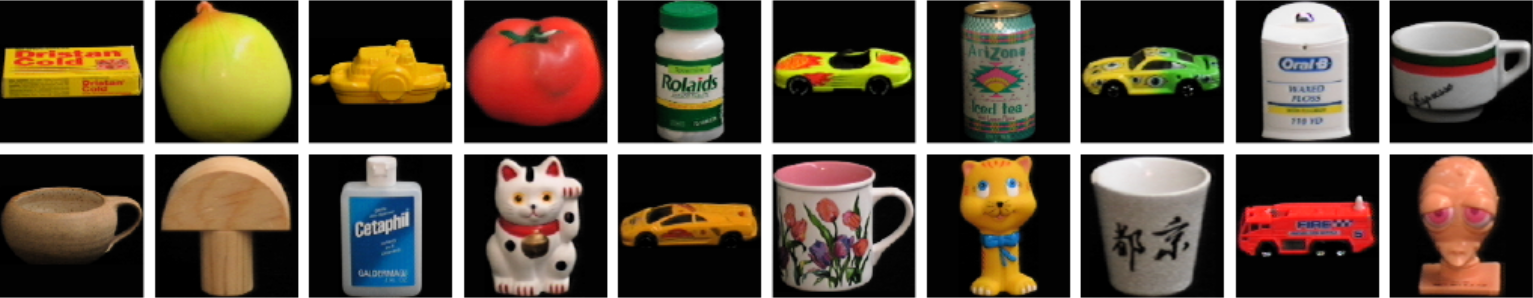
\includegraphics[width=1\textwidth]{coil100}
	\caption{A subset of 20 objects taken from the COIL100 dataset.}
	\label{fig:coil100_objects}
\end{figure}
In order to be able to present the learning algorithm many different views on one single object, the camera took a photo of the rotating object, each time it has turned by 5 degrees, yielding 72 images per object and 7200 in total. Since the creators of the dataset do not provide or suggest any established separation in training and test data, we created those sets on our part, randomly dividing the 72 images of each object into 54 training images and 14 test images, totalling in 5400 training images and 1400 test images.\\
Since the provided images are already cropped in a reasonable manner, unlike the images of the GTSRB dataset, we did not crop the images any further. However, we were obliged to rescale the images to a size of $48 \times 48$ pixels to fit the structure of the adopted GTSRB CNN; otherwise we would not have been able to reuse the filters trained on the GTSRB network, because the filter sizes for the COIL100 network would not match the ones, which have already been trained before for the GTSRB network. Since we had found that distorting the images before each training epoch had improved the results, we applied the distortions also to the images of this dataset.

\subsubsection{Results with reused GTSRB filters}

The green curve in figure \ref{fig:coil100_results} illustrates the results on the test set, which we achieved by letting the weights of the convolutional layers unchanged and training only the randomly initialized weights of the fully connected layers. The column "GTSRB filters" in table \ref{tab:coil-results} provides the exact numbers. We observe that the accuracy increases monotonically until the eighth epoch, where we obtained a result of 100\%. The following decrease of the recognition rate can be explained as a consequence of the randomized distortions, which are applied before each epoch. Howsoever, the accuracy does not decrease by a large amount (an accuracy of 99.93\% indicates one misclassfied image, 99.79\% indcate three misclassified images) and stabilizes again at 100\% after 14 epochs. Training one epoch lasts about 300 seconds. Thus, it is possible to construct a reliable classifier for this task in a short time interval by reusing pre-trained filters from another network.%TODO Add information about zappa02 processor ecc.
\begin{figure}[h!]
	\centering
	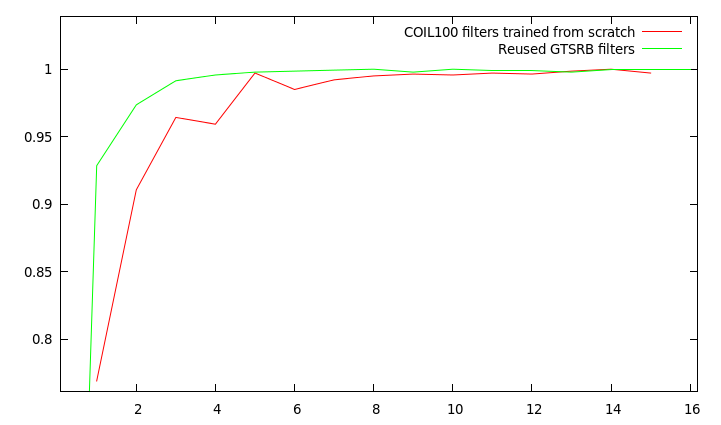
\includegraphics[width=1\textwidth]{coil100_results.png}
	\caption{Results on the COIL100 dataset with filters completely trained from scratch and with reused GTSRB filters.}
	\label{fig:coil100_results}
\end{figure}
\begin{table}[h!]
	\centering
	\begin{tabular}{|r|rr|}
		\hline
		Epoch & GTSRB Filters & Fresh Filters\\ \hline
		00 & 0.02500 & -\\
		01 & 0.9286 & 0.7693\\
		02 & 0.9736 & 0.9107\\
		03 & 0.9914 & 0.9643\\
		04 & 0.9957 & 0.9593\\
		05 & 0.9979 & 0.9971\\
		06 & 0.9986 & 0.9850\\
		07 & 0.9993 & 0.9921\\
		08 & 1.0000 & 0.9950\\
		09 & 0.9979 & 0.9964\\
		10 & 1.0000 & 0.9957\\
		11 & 0.9993 & 0.9971\\
		12 & 0.9993 & 0.9964\\
		13 & 0.9979 & 0.9986\\
		14 & 1.0000 & 1.0000\\
		15 & 1.0000 & 0.9971\\ \hline
	\end{tabular}

	\caption{Results on the COIL100 dataset with reused GTSRB filters and fresh filters.}
	\label{tab:coil-results}
\end{table}

\subsubsection{Results with randomly initialized filters}

In addition, we set up a network with the same structure, but initialized the weights of all layers randomly. The results of this setup are illustrated by the red curve in figure \ref{fig:coil100_results} and the column "Fresh Filters" in table \ref{tab:coil-results}.

\begin{figure}[h!]
	\centering
	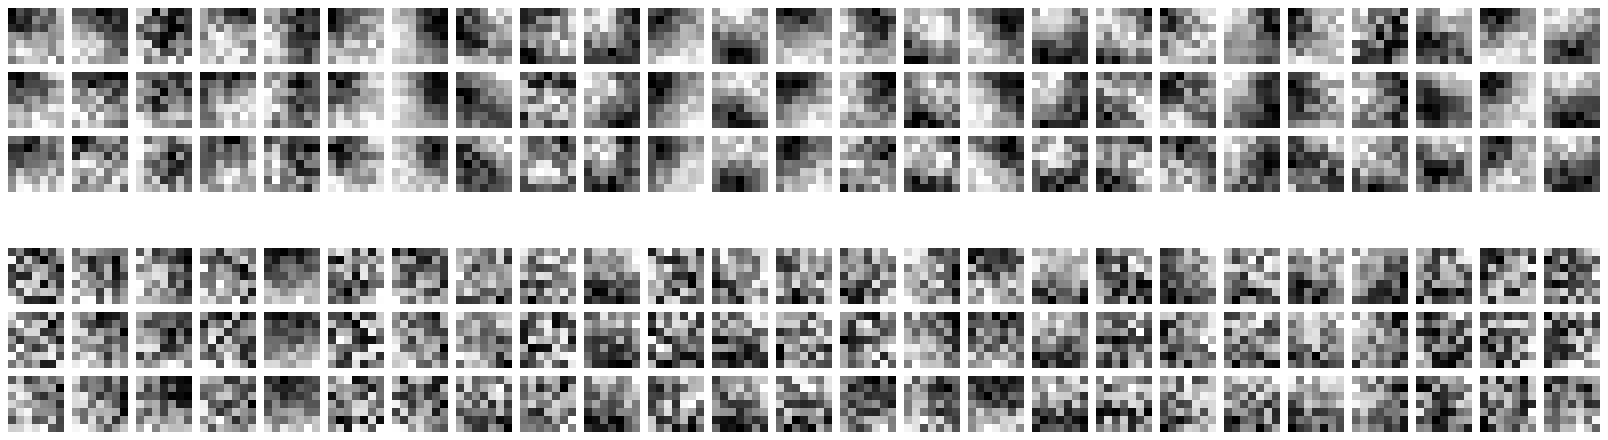
\includegraphics[width=1\textwidth]{gtsrb_vs_coil_filters.png}
	\caption{Filters of the first 25 maps from the input layer to the second layer. The upper filters are taken from the GTSRB CNN after 12 epochs of training, the lower filters are taken from the COIL100 CNN after 15 epochs of training. The three rows show the filters for the red, green and blue channel respectively.}
	\label{fig:gtsrb_vs_coil_filters}
\end{figure}


\subsection{INRIA dataset}

After achieving excellent results on the COIL100 dataset, we tried to get similar results on a probably more difficult dataset. The dataset we chose is the Head Pose Image Database \cite{estimating-face-orientation-inria} from the French Institute for Research in Computer Science and Automation (INRIA). The dataset consists of 15 persons, two series per person and 93 JPEG-images per series. In each series the depicted person changes its head posture gradually. One of the two series shows the person with a certain feature like glasses, the other series does not. Figure \ref{fig:inria_different_angles} shows some example images for one person taken from one series.

\begin{figure}[h!]
	\centering
	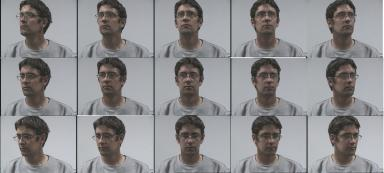
\includegraphics[width=0.8\textwidth]{inria_different_angles}
	\caption{Person 12 presented from different angles.}
	\label{fig:inria_different_angles}
\end{figure}

The problem appears to be harder than the COIL100 problem, because the persons in the INRIA dataset are more similar to each other than the objects in the other dataset.

\begin{figure}[h!]
	\centering
	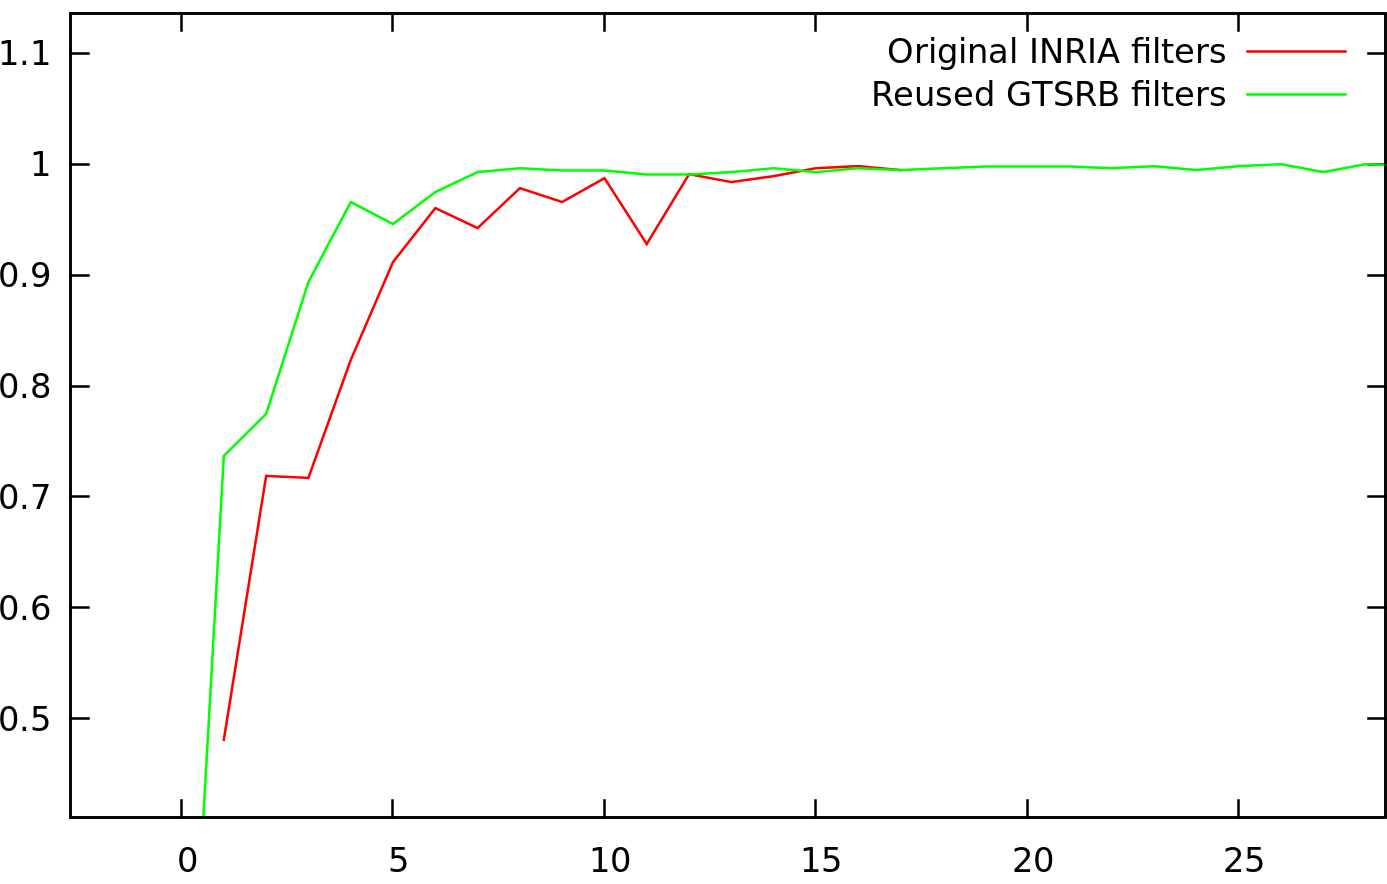
\includegraphics[width=1\textwidth]{inria_results.png}
	\caption{Results on the INRIA dataset with filters completely trained from scratch and with reused GTSRB filters.}
	\label{fig:inria_results}
\end{figure}

\begin{appendix}
	\section{Implementation}
	
	\subsection{Keras, etc...}
	
	\subsection{Distortions}
	% TODO be precise about the input being distorted before the first epoch.
	
	\label{sec:implementation-distortions}
	\section{Visualization}
\end{appendix}

\addcontentsline{toc}{section}{References}
\bibliography{ref}{}
\bibliographystyle{alpha}

\end{document}






